\chapter{INTRODUCTION}

\section{Project Scope and Context: The Digital Transformation of Live Events}

The rapid evolution of technology is a driving force for the development of businesses in the food service industry. This is achieved through the gradual introduction of smart business management systems. A business must be able to respond to customer needs for high-quality service and immediate responsiveness, while simultaneously achieving optimal resource utilization and cost reduction. This is particularly important in the context of temporary events and festivals, where resources are limited and the environment is highly demanding. The obvious solution to these challenges is the introduction of a smart order management system (OMS). An OMS enables effective order management through automation, optimal resource allocation, and savings in time and money. The implementation of an OMS for supporting temporary events or music festivals proves to be particularly attractive and effective. Therefore, in order to function, modern events create temporary digital ecosystems that rely on digital interactions.

On the other hand, the back-end of large-scale temporary events such as three to four-day music festivals, trade shows and exhibitions, and conference ``pop-ups'' are a hostile environment for traditional ICT solutions. Unlike the always-on access to high-speed broadband found in typical, permanent hospitality settings, such as restaurants and hotels, these environments can be supported by a combination of satellite uplinks, microwave point-to-point links, and mobile cell towers for network access. These mobile cell towers are designed for occasional, short-term use by thousands of people using mobile phones to upload videos, etc. Thus, the electromagnetic environment surrounding these cell towers is congested and limited by the available spectrum. There are latency spikes, high packet loss, and variable connectivity \cite{ibm2019cloud}.

This research takes place at the crossroads of high-performance web application development and the anthropological, chaotic, and unpredictable world of event-based networking. Over the last five years, we have witnessed the growth of cloud-native development. Cloud-native development promotes the use of thin-client, local applications that continuously interact with centralized remote servers to provide business logic. While thin-client architectures are successful in a reliable enterprise environment, they are severely restricted and fragile in an event environment where the number of delegates accessing the local wireless network can easily overwhelm the network. If a typical cloud-first POS system received too many requests from the thousands of individuals in the building utilizing the wireless network, it would time-out all transaction requests. Similarly, if the cashier's tablet could not contact the cloud-server to validate the transaction, the system would freeze, causing the entire service to be unavailable and resulting in lost potential revenue from the event.

This dissertation will provide a comprehensive, detailed presentation of the physical implementation and extensive evaluation of a new, high-performing Order Management System (OMS). The specific use-case of the proposed OMS will be designed to accommodate the extreme conditions inherent to temporary event environments. This proposed POS system will be a robust, locally-centric, distributed application utilizing current web technologies (i.e., the MERN Stack). The proposed POS system will utilize the latest web technologies in a unique way, by deploying the web technologies within a closed, containerized, internal network, on-site. As such, regardless of the status of the external internet, all critical financial transactions, inventory reductions, and critical messages to the kitchen will be real-time, fully functional, and completely synchronized.

\subsection{The Historical Evolution of Order Management Systems}

To better understand the need for this local architecture, we have to look at the historic development of point-of-sale (POS) technology. The original point-of-sale system was large mechanical cash register that was connected to no other data resource. It was extremely robust, but provided managers with none of the current real-time information about their business. Managers did not know which products sold out nor how much money they made until the long, arduous task of manually counting the cash at the end of each day.

The next generation of technology provided the first localized network systems, commonly called electronic point-of-sale (EPOS) systems. EPOS systems brought all of the terminals at a single site online and passed the sales data to a server located in the back office. Although EPOS systems resolved the issue of aggregating sales data in real time, the previous EPOS systems were very inflexible, extremely expensive to license, and required high levels of technical expertise to make simple menu changes.

Currently, the dominant model of POS technology has been to implement cloud-based POS applications using inexpensive off-the-shelf devices such as Apple iPads and then connect those devices to massive cloud servers maintained by third parties. Cloud-based POS solutions have dramatically lowered the cost of accessing enterprise-level analytical capabilities and greatly simplified remote management. However, as described above, this approach has significant trade-offs related to local control, and the ability of a business to operate will be directly tied to the reliability of an external internet connection. As many festivals are either held in remote locations or temporary locations with limited connectivity, this is a major problem. The primary focus of this dissertation is to architecturally synthesize the best features of both approaches. In other words, to create a system that provides the extreme administration flexibility and intuitive user experience of today's cloud-based applications, while still providing the same type of reliable operation that we have come to expect from our EPOS systems. This historical progression of operational architectures is visually summarized in Figure~\ref{fig:pos_evolution}.

\begin{figure}[htbp]
    \centering
    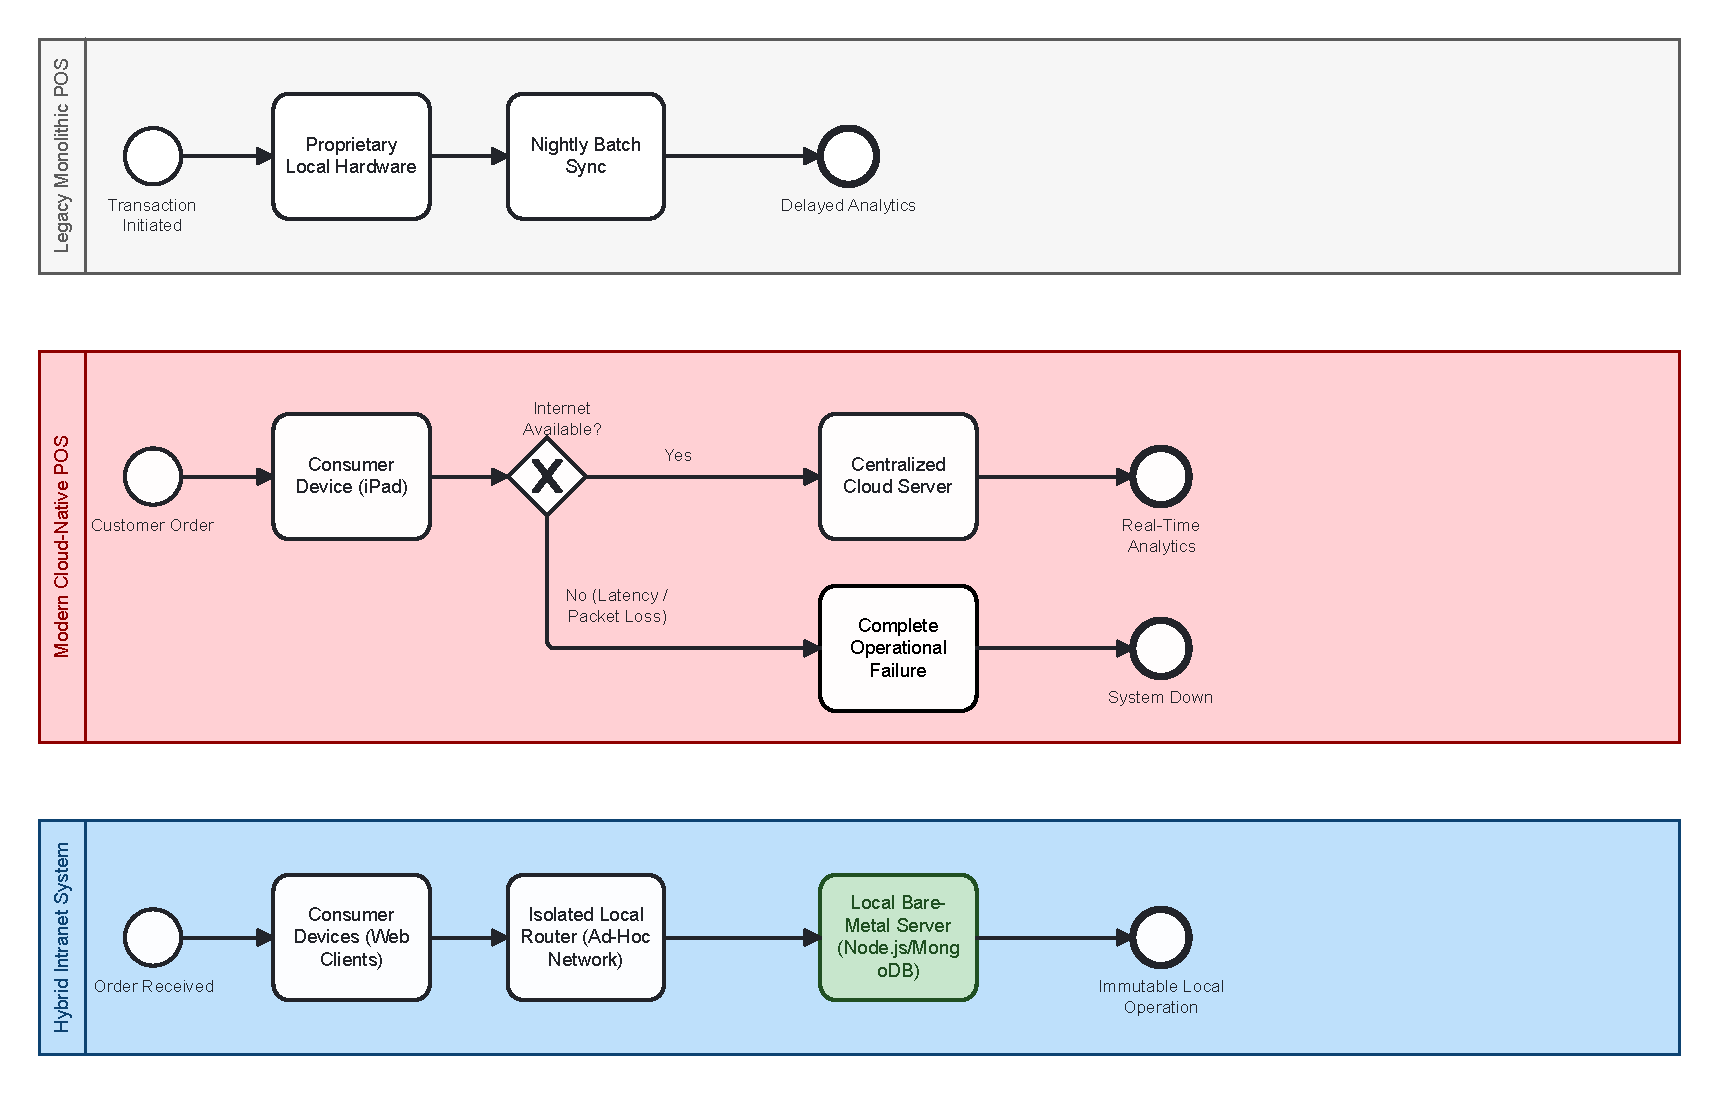
\includegraphics[width=0.9\textwidth]{images/ch1_pos_evolution.pdf}
    \caption{The architectural evolution of Point of Sale systems from mechanical isolation to local-first decentralized networks.}
    \label{fig:pos_evolution}
\end{figure}

\section{Problem Statement: Challenges in Ad-Hoc Networks}

Today, digital order systems are widely used in the food service sector due to the benefits they offer to businesses. However, applying them to temporary environments poses specific challenges due to non-permanent infrastructure, massive customer volumes, low-quality networks, and the need for real-time execution.

\subsection{Common Operational Challenges}
To be both successful and effective in a high-volume process, speed of raw processing is essential. Based on queue theory, as the service rate (the speed at which the items being ordered are served) is significantly less than the arrival rate (the speed at which patrons enter the queue for an item), the service rate is negatively affected as the average service time increases. The smallest delay between transmitting information and receiving it on the network may result in significant issues.

Currently, most systems utilizing traditional web protocols utilize an explicit request/response model. An example of this occurs when an individual requests to purchase a ticket. The request will take hundreds of milliseconds to travel from the ticket-buying tablet located at the cash register via the nearest access network (e.g., mobile cellular network), through the internet backbone, to the cloud server for processing. Once the request has been processed, the response will travel back to the tablet. As previously mentioned, although the time delay stated may appear small and tolerable for most users of the internet at home with a typical computer to complete an e-commerce transaction, this is a large problem when operating in a bar or other high pressure environment.

Although this does not appear to be a problem when the shop is not busy, it is a very bad problem as queues of customers build up and is a direct manifestation of network-induced latency degradation under concurrent load \cite{ibm2019cloud}. As the shopping experience becomes busier, the number of transactions becomes exponentially greater. Another problem encountered by users is when the Point of Sale (POS) interface freezes on a screen and users repeatedly hit the ``confirm payment'' button, thereby inducing race conditions on the server. These race conditions have caused unintended duplicate charges to consumers and catastrophic discrepancies in financial reporting. 

In addition to the previous issue of unintended duplicate charges, data corruption is another, similar, and critical issue that can occur when there are unannounced and temporary network communication problems such as packet loss. For example, when a POS terminal sends a payment confirmation to the central servers of a payment platform. The server processes the transaction, stores it in the database, and then sends an acknowledgement packet back to the POS terminal. Due to heavy local Wi-Fi interference, the acknowledgement packet never reaches the terminal and is lost. 

The server has received and processed the transaction entered, and recorded it in the database. The POS terminal has timed out while waiting for the delayed response packet. The cashier must read the error response at the POS terminal, either re-charge the credit card through logical cashier or ask the customer to pay through another method. In both cases, there will be lost sales, unhappy customers, inefficient operations, possible litigation, or worst case scenario, the cashier may frantically try to keep lines of customers moving by canceling a good electronic transaction just so he can clear an error message. In either case, canceling the transaction will result in incorrect logged inventory and inaccurate daily metrics. 

The previous examples are standard examples used in abstract distributed computing, the so-called ``Two Generals Problem.'' In a computer system, the Two Generals Problem is a theoretical thought experiment that shows the impossibility of perfect synchronization between two autonomous computer systems over an unreliable communications channel \cite{brewer2012cap}. If the communications channel also is unreliable, the computer system cannot detect receipt of packets, unless a reliable hand-shaking protocol is utilized. The above naive design principles and the simple models of eventual consistency that typify many cloud applications are fundamentally inadequate to meet the higher reliability requirements for real-time financial offline accounting in extreme field environments. This profound conceptual communication dilemma is conceptualized in Figure~\ref{fig:two_generals}.

\begin{figure}[htbp]
    \centering
    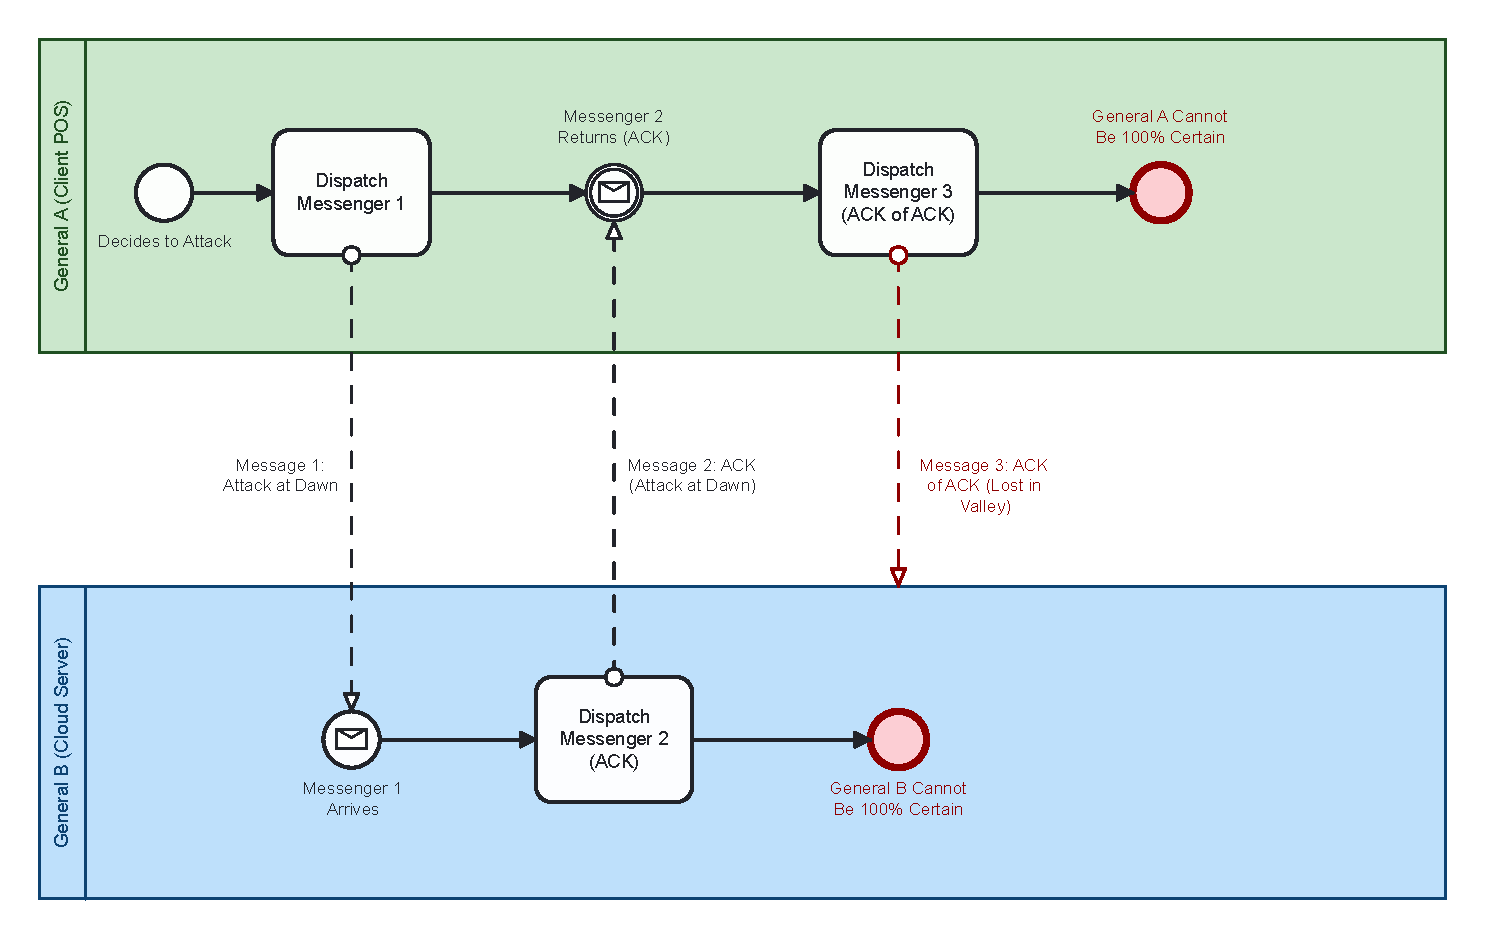
\includegraphics[width=0.8\textwidth]{images/ch1_two_generals.pdf}
    \caption{Visualizing the Two Generals Problem: Achieving deterministic synchronized state over an unreliable ad-hoc network connection.}
    \label{fig:two_generals}
\end{figure}
\section{Research Objectives}

The primary objective of this thesis is the design and implementation of a flexible, user-friendly, and efficient Order Management System (OMS). The specific sub-objectives of the system include: for supporting high transaction loads during temporary events, achieving low network latency, ensuring optimal resource utilization, maintaining high reliability and resilience, minimizing service time for faster customer processing, and effectively managing burst order scenarios.

To address the aforementioned objectives, it is necessary to remove the synchronous request-response paradigm and utilize the highly optimized, persistent, full-duplex communications channels provided by WebSockets \cite{fette2011websocket, mdn2023websocket}.

In addition to the aforementioned, a second major goal of the thesis is to provide strong deterministic guarantees of the absolute consistency of all information contained within every node in the system and to eliminate the extremely deleterious phenomenon of phantom orders. Each node in the system must verify via strict validation on the database side that there exists no state of visual confirmation of the completion of an order by the frontend operator that has occurred until all transactional data has been safely stored and permanently recorded into the persistent ledger on the backend server computer system.

In addition, the design of the system must include the ability to maximize transaction throughput that can be supported concurrently by the system in the most efficient manner possible, while maintaining the highest level of data consistency and eliminating the phantom order issue. Thus, the system must be capable of supporting a minimum of 50 concurrent client devices hammering the system simultaneously, and more than 1,000 complex transactions per hour. Moreover, the system must be able to achieve this level of throughput on a single low-power commodity hardware server (such as an Intel NUC or commodity laptop), to maintain the economic viability of the solution and affordability for individual event organizers who have limited budgets.

Finally, the system is expected to greatly enhance management's operational insights by providing real-time, reactive dashboards as a feedback mechanism. The dashboards will periodically report on sales rates, the current live depletion of each item of inventory, and the performance of individual staff members. Unlike conventional cash registers, which accumulate vast amounts of un-invoiced data dumps in the back office to be reviewed during nightly reconciliation, the system data will be immediately accessible to managers for in-event analysis, enabling them to dynamically allocate staff to busy sections of the venue and suspend the sale of depleted stock items.

\section{Scope and Limitations}

This project focuses on the design and development of a high-throughput order management application tailored for large-scale events, aiming at the efficient entry, processing, and tracking of orders in real-time.

In addition to developing the full software stack of MongoDB, Express.js, React.js and Node.js \cite{banker2011mongodb, express, freeman2019pro, tilkov2010node}, the project will build the deep technical design of the LAN architecture and the strong real-time signal protocol necessary to operate reliably in hostile mission environments. Also, the project will develop multiple modules that support different roles, such as cashier, administrator and kitchen staff, and will implement an advanced algorithmic user authentication system and role-based access controls using a middleware solution on the server-side.

There are a number of large-scale aspects of this project that have been excluded from the scope of the project. Examples of these large-scale aspects include the development of native mobile apps for iOS and Android. Instead of developing native mobile apps for iOS and Android, the project will focus on developing a highly optimized progressive web application (PWA) that can run on most modern standard web browsers \cite{google2020offline}. The choice of PWA technology allows for maximum cross-platform device compatibility with minimal setup/approval requirements from app stores.

However, the project has intentionally avoided the detail low-level engineering of a completely certified, PCI-DSS compliant credit card processing gateway. Lastly, the project assumes that the infrastructure will be built around off-the-shelf consumer tablets and standard IP thermal ticket printers. Therefore, the project will exclude the manufacturing process for creating custom physical hardware.

\section{Thesis Structure}

This portion of the dissertation has been structured in a manner that will allow for a detailed examination of the solution by using a methodical approach. Chapter 2 (Theoretical Background and Technologies) provides the academic base to support the development of the solution based on the models and architectures required to develop high load systems. Chapter 3 (Requirements Analysis and System Design) translates the architectural design as defined by the theoretical components into strict architectural definitions, including an evaluation of the users that will utilize the system, the functional requirements that the system must meet, and the structure of the data. Chapter 4 (Information System Implementation) details the concrete implementation of the backend subsystem, frontend interfaces, and security middleware integration. Chapter 5 (Experimental Evaluation and Empirical Analysis) presents the comprehensive experimental assessment, including comparative baseline studies, stress testing, automated functional verification, and field study analysis. Finally, Chapter 6 (Conclusions and Future Work) summarizes the major technological accomplishments and outlines possible directions for future research and architectural expansion.